\chapter{Εφαρμογή Αλγορίθμων Διαφορικής Ιδιωτικότητας}


Στο κεφάλαιο αυτό θα περιγράψουμε τη δημιουργία προγραμμάτων ανωνυμοποίησης, χρησιμοποιώντας μηχανισμούς Διαφορικής Ιδιώτικότητας. Στη συνέχεια κάνουμε χρήση των αλγορίθμων αυτών με επερωτήσεις πάνω σε σύνολα δεδομένων. Τέλος εξάγουμε συμπεράσματα από την εφαρμογή των μηχανισμών. 

\section{Υλοποίηση}

 Η αρχιτεκτονική των μοντέλων που διαχειρίζονται τους μηχανισμούς τυχαιοποίησης είναι εντελώς διαφορετική από αυτήν των μηχανισμών γενίκευσης που αναλύσαμε. Όπως είδαμε στο κεφάλαιο 3, η τεχνική που χρησιμοποιούν οι περισσότεροι αλγορίθμοι είναι να δέχονται ένα σύνολο δεδομένων, και να επιστρέφουν μια ανωνυμοποιημένη εκδοχή του. Σε αυτή τη νέα βάση εργάζονται στη συνέχεια οι αναλυτές. Η χρήση διαδραστικών τεχνικών απαιτεί διαφορετική μοντελοποίηση: Από την μια μεριά, ο αναλυτής θέτει την επερώτησή του στην βάση δεδομένων, ενώ από την άλλη ο διαχειριστής επιλέγει το μέγεθος ιδιωτικότητας που επιθυμεί\footnote{Επιλογή της παραμέτρου $\epsilon$}. Τα δεδομένα επεξεργάζονται, προστίθεται ο θόρυβος και το αποτέλεσμα επιστρέφει στον αναλυτή.

Στο πρόγραμμα μας, θα κάνουμε χρήση κυρίως του μηχανισμού \textlatin{Laplace}, ο οποίος ικανοποιεί το κριτήριο της ΔΙ όπως δείξαμε στο προηγούμενο κεφάλαιο. 

Η συνάρτηση πυκνότητας πιθανότητας για μέσο $\mu=0$ είναι 
$$f(x|0,b)=\frac{1}{2b}e^{-\frac{|x|}{b}}$$

άρα έχουμε την αθροιστική συνάρτηση κατανομής:
$$F(x)=
\int_{-\infty}^{x} f(u)du=
\int_{-\infty}^{x} \frac{1}{2b}e^{-\frac{|u|}{b}}du=
 \begin{cases} 
      \frac{1}{2}e^{\frac{x}{b}} & x< 0 \\
      1-\frac{1}{2}e^{\frac{-x}{b}} & x\geq 0 
   \end{cases}$$
Η αντίστροφη συνάρτηση είναι:
$$F^{-1}(x)=
\begin{cases} 
      b\cdot ln(2x) & 0<x<1/2 \\
      -b\cdot ln(2-2x) & 1/2 \leq x \leq 1
   \end{cases}$$
 Θέτωντας $u=x-1/2$ καταλήγουμε σε μια γεννήτρια τυχαίων μεταβλητών:
$$X=-b\cdot sgn(u)ln(1-2|u|) \quad u\in \Big(-\frac{1}{2}, \frac{1}{2}\Big]$$

Έτσι, επιλέγοντας τυχαίες μεταβλητές $u$ από την ομοιόμορφη κατανομή στο διάστημα  $[-0.5, 0.5]$ , η τυχαία μεταβλητή $X$ θα ανήκει στην κατανομή \textlatin{Laplace} με παράμετρο κλίμακας $b$. 

Κατασκευάζουμε δυο διαφορετικές συναρτήσεις. Η μια ως είσοδο δέχεται παράμετρο $b$ και πλήθος μεταβλητών που επιθυμούμε, ενώ η δεύτερη την παράμετρο $\epsilon$ και διάσταση βάσης δεδομένων.
H σχέση που συνδέει το $\epsilon$ με την παράμετρο $b$ είναι 
$$b=\frac{\Delta f}{\epsilon}$$
με $\Delta f$ να συμβολίζει την ευαισθησία  μιας συνάρτησης $f:X \longrightarrow \mathbb{R}^k:$

$$\Delta f=max_{x\sim x'}||f(x)-f(x')||$$
όπου $x,x'$ δύο γειτνιάζουσες βάσεις δεδομένων\footnote{
Σε περίπτωση που απαιτηθεί αυστηρή εφαρμογή του ορισμού της ευασθησίας: Για την δημιουργία της βάσης $x'$, έχουμε αναπτύξει την συνάρτηση «\textlatin{falsedata}», η οποία έχει ως είσοδο την αρχική βάση $x$ και ως έξοδο μια νέα βάση η οποία διαφέρει από την αρχική το πολύ σε μια εγγραφή. Η συνάρτηση επιλέγει τυχαία μια πλειάδα της βάσης, και μεταβάλει τις τιμές των αντίστοιχων γνωρισμάτων με τυχαίο τρόπο:
\begin{itemize}
    \item Για αλφαριθμητικά γνωρίσματα, επιλέγει μια τιμή από το πεδίο τιμών του αντίστοιχου γνωρίσματος.
    \item Για αριθμητικά γνωρίσματα, η συνάρτηση εντοπίζει την ελάχιστη και την μέγιστη τιμή του γνωρίσματος και επιλέγει μια τυχαία τιμή σε αυτό το διάστημα. Έτσι διασφαλίζεται η επιπλέον διατήρηση της ιδιωτικότητας ειδικά αν αυτό το γνώρισμα είναι ευαίσθητο.
    \item Για τα λογικά γνωρίσματα (στην περίπτωση της δικής μας βάσης, οι τιμές είναι \textlatin{YES} ή \textlatin{NO}),
    επιλέγεται τυχαίως μια εκ των δύο τιμών, αλλά με πιθανότητα αντίστοιχη της εμφάνισης στη βάση. Δηλαδή αν το γνώρισμα παίρνει τις τιμές 0 ή 1, και οι άσσοι είναι 9πλάσιοι από τα μηδενικά, θα επιλεγεί η τιμή 1 με πιθανότητα 90\%. 
\end{itemize}
}.




\clearpage
Το σύνολο δεδομένων που χρησιμοποιούμε στα πειράματα είναι ένας πίνακας εκπαιδευτικών ΠΕ19 Πληροφορικής του Υπουργείου Παιδείας\footnote{\textlatin{\url{http://e-aitisi.sch.gr}}}. Αφού μετατρέψαμε τους χαρακτήρες από ελληνικά σε λατινικά, αφαιρέσαμε περιττά και ευαίσθητα γνωρίσματα. Καταλήγουμε στην τελική μορφή ενός συνόλου δεδομένων που αποτελείται από 1400 περίπου εγγραφές και έχει τα γνωρίσματα \{Όνομα, Μόρια, Παιδαγωγικό, Βαθμός, Τρίτεκνος\}. Συγκεκριμένα:
\begin{itemize}
    \item Όνομα: Το μικρό όνομα του ατόμου
    \item Μόρια: Τα μόρια που έχει συγκεντρώσει (θεωρείται ευαίσθητο χαρακτηριστικό)
   \item Παιδαγωγικό: \textlatin{YES} Αν διαθέτει παιδαγωγική πιστοποίηση, \textlatin{NO} διαφορετικά.
   \item Βαθμός: Βαθμός πτυχίου (θεωρείται ευαίσθητο χαρακτηριστικό)
   \item Τρίτεκνος: \textlatin{YES} Αν έχει τρία παιδιά τουλάχιστον, \textlatin{NO} διαφορετικά.
    
    
\end{itemize}


\begin{figure} [ht]
\begin{center}
  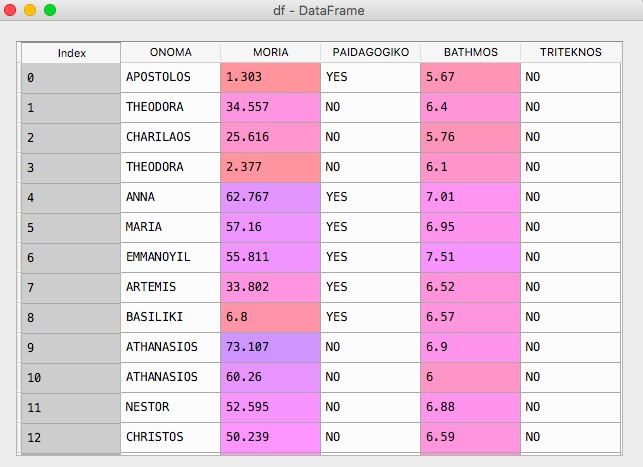
\includegraphics[scale=0.55]{images/DF.jpg}
  \caption{Πίνακας αναπληρωτών εκπαιδευτικών ΠΕ19, μετά από ανωνυμοποίηση.}
  %\label{fig:boat1}
  \end{center}
\end{figure}


Η επιλογή της βάσης έγινε λόγω των χαρακτηριστικών της, τα οποία θα μας καλύψουν στους υπολογισμούς που επιθυμούμε να πραγματοποιήσουμε. Επιπλέον, το μεγέθος είναι ιδανικό για να εμφανιστούν τυχόν σφάλματα από κακή επιλογή παραμέτρων. 






\clearpage
\section{Εφαρμογή και αξιολόγηση}

Η ανάπτυξη του αλγορίθμου γίνεται σε γλώσσα \textlatin{Python}, έκδοσης 2.7.15, σε σύστημα \textlatin{OS X} υπολογιστή \textlatin{Mac}, με διπύρινο επεξεργαστή συγχρονισμένο στα 2.4 \textlatin{GHz}. Κάνουμε χρήση των βιβλιοθηκών $Numpy$  kαι $Pandas$, ενώ η υλοποίηση γίνεται στο περιβάλλον προγραμματισμού  \textlatin{Spyder}.
 

\subsection{Δημοφιλή ονόματα}

Στο πείραμα αυτό θα εφαρμόσουμε την επερώτηση "ποιό είναι το πιο συνηθισμένο όνομα στη βάση δεδομένων?".

Υλοποιούμε μια συνάρτηση που δεχεται ως όρισμα την βάση δεδομένων, μετρά το πλήθος του κάθε ονόματος και επιστρέφει αυτό με την μέγιστη τιμή. Υλοποιούμε και μια συνάρτηση τυχαιοποίησης, που δέχεται ως όρισμα την βάση και την παράμετρο $\epsilon$ και πραγματοποιεί ακριβώς την ίδια διαδικασία, αλλά στο τέλος προσθέτει θόρυβο από την κατανομή \textlatin{Laplace}.

Η ευαισθησία της επερώτησης θα είναι $\Delta_f=1$, οπότε η παράμετρος κλίμακας της \textlatin{Laplace} είναι $b=\frac{1}{\epsilon}$.

Για $\epsilon=1$ έχουμε το αποτέλεσμα:
\begin{itemize}
    \item Χωρίς θόρυβο: '\textlatin{GEORGIOS}'
     \item Με θόρυβο: '\textlatin{GEORGIOS}'
\end{itemize}



Για $\epsilon=0.4$, μετά από λίγες εκτελέσεις προκύπτει το αποτέλεσμα:
\begin{itemize}
    \item Χωρίς θόρυβο: '\textlatin{GEORGIOS}'
     \item Με θόρυβο: '\textlatin{MARIA}'
\end{itemize}

Οπότε επαληθεύουμε την πρόταση ότι όσο μικραίνει η τιμή του $\epsilon$, τόσο η απώλεια πληροφορίας μεγιστοποιείται. 

Επεκτίνουμε την επερώτηση, αναζητώντας περισσότερα του ενός ονόματα. Η επερώτηση μας είναι τύπου Ιστογράμματος (\textlatin{histogram query}), οπότε εξακολουθεί η ευαισθησία να έιναι $\Delta_f=1$. Επιλέγουμε λοιπόν να υπολογιστούν τα 12 δημοφιλέστερα ονόματα στη βάση , επιλέγοντας $\epsilon=1$.

\begin{figure} [ht]
\begin{center}
  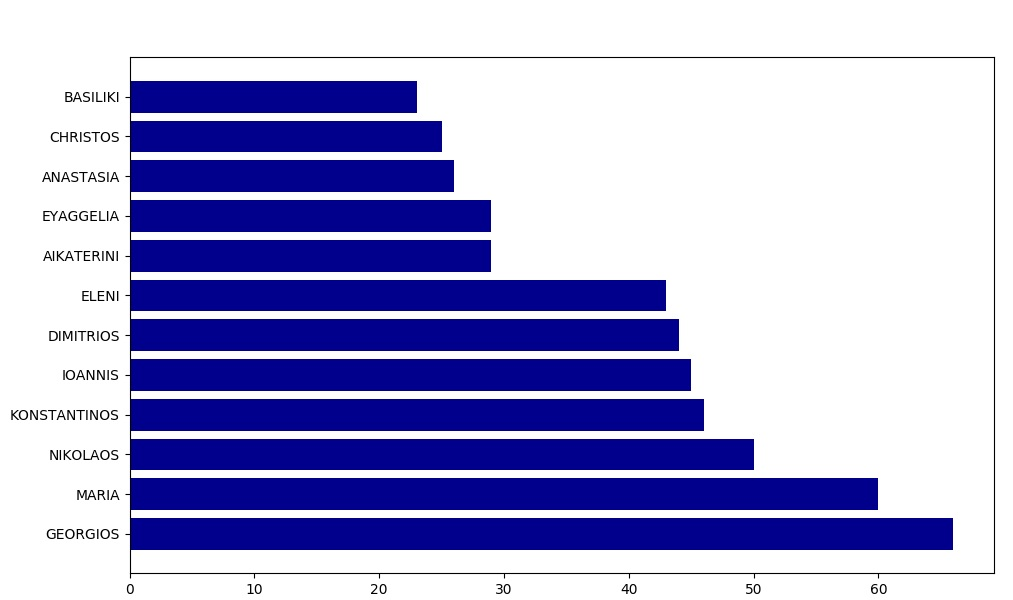
\includegraphics[scale=0.41]{images/e=1.jpg}
  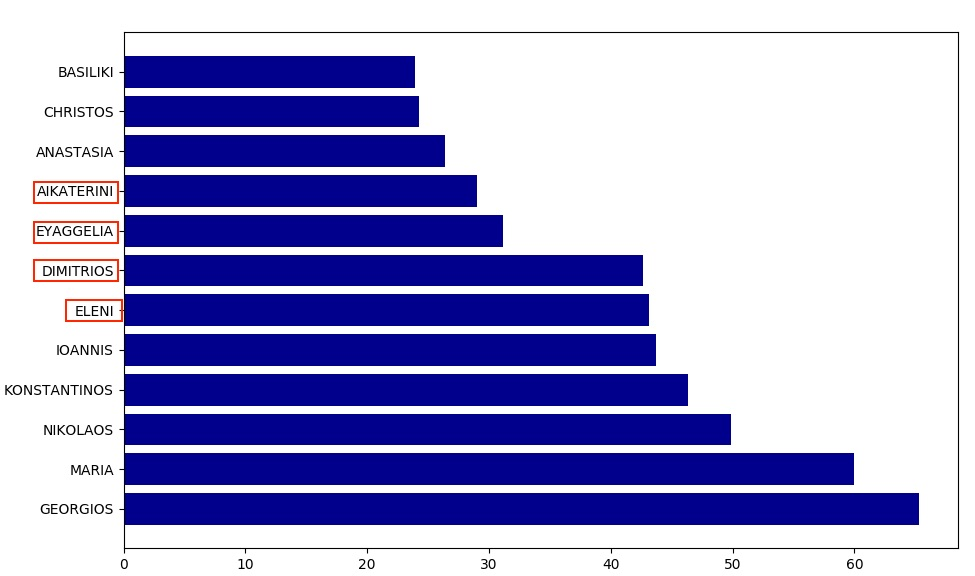
\includegraphics[scale=0.41]{images/e=2.jpg}
  \caption{Δημοφιλέστερα ονόματα - χωρίς θόρυβο (πάνω) και με θόρυβο (ε=1) (κάτω)}
  %\label{fig:boat1}
  \end{center}
\end{figure}

Παρατηρούμε ότι η πρώτη τριάδα παραμένει ανεπηρέαστη. Αντίθετα στις μεσαίες τιμές, όπου οι συχνότητες των ονομάτων είναι αρκετά κοντά, παίρνουμε εσφαλμένα αποτελέσματα. Έκτο δημοφιλέστερο όνομα στην βάση προκύπτει το '\textlatin{ELENI}', αντί του πραγματικού '\textlatin{DIMITRIOS}', παρά το ότι στην εκτέλεση της αρχικής επερώτησης η επιλογή του $\epsilon$ να έχει την τιμή 1 ήταν αποτελεσματική.

Αντιλαμβανόμαστε το μέγεθος του ζητήματος για την ορθή επιλογή της παραμέτρου $\epsilon$, το οποίο οφείλει να προβάλει τα αποτελέσματά των επερωτήσεων σε απόλυτη ισορροπία: διατηρώντας την ιδιωτικότητα των δεδομένων του συνόλου και διασφαλίζοντας την ακρίβεια του αποτελέσματος.




\subsection{Μέση τιμή}

Στο πείραμα αυτό θα εφαρμόσουμε διάφορες μορφές της κλασικής επερώτησης για την εύρεση της μέσης τιμής ενός ευαίσθητου, αριθμητικού χαρακτηριστικού.

Ξεκινάμε με την εύρεση της μέσης τιμής του γνωρίσματος '\textlatin{BATHMOS}'. Θα έχουμε λοιπόν:
$$f(x)=\frac{1}{n}\sum_{i=1}^n b_i$$

Οι τιμές των βαθμών κειμένονται στο διάστημα $[5, b_{max}]$. Παρατηρούμε ότι $$|b_i - b_i'|\leq b_{max}-5$$, συνεπώς η ευαισθησία μπορεί να υπολογιστεί ως εξής:
$$\Delta_f=max_{x\sim x'}|q(x)-q(x')|=\frac{1}{n}max_{x_i,x'_i}|b_i - b'_i|\quad  i \in [1,n]$$
Έτσι έχουμε
$$\Delta_f=\frac{b_{max}-5}{n}$$
Γνωρίζουμε ότι ο μηχανισμος
$$M(x)=\frac{\sum_{i=1}^{n}b_i}{n}+Lap(\frac{b_{max}-5}{n\epsilon})$$
θα διατηρεί $\epsilon$-διαφορική ιδιωτικότητα\textlatin{\cite{dp2}}. Εφαρμόζοντας τον τύπο στους υπολογισμούς μας παίρνουμε τα αποτελέσματα για τον μέσο βαθμό

\begin{itemize}
    \item Αρχικά: 6.74
    \item Με $\epsilon=1$: 6.74
    \item Με $\epsilon=0.1$: 6.73
    \item Με $\epsilon=0.01$: 6.81
\end{itemize}


Μια άλλη εκδοχή, είναι να προσθέσουμε θόρυβο \textlatin{Laplace} σε κάθε έναν από τους βαθμούς και να υπολογιστεί στη συνέχεια η μέση τιμή τους. Λόγω του θεωρήματος της σύνθεσης ικανοποιείται η $\epsilon$-διαφορική ιδιωτικότητα. Με αυτόν τον τρόπο μπορούμε να απεικονίσουμε και το ιστόγραμμα συχνοτήτων των βαθμών.

\begin{figure} [ht]
\begin{center}
  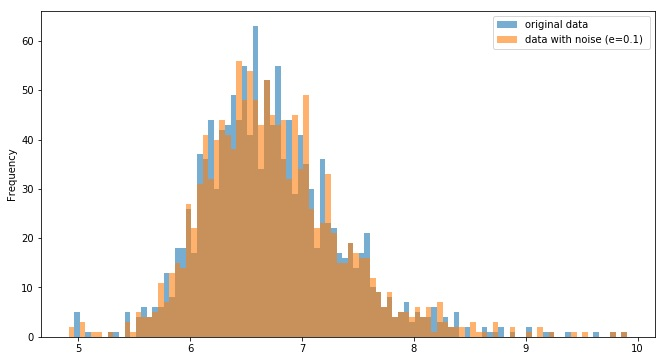
\includegraphics[scale=0.59]{images/hist01.jpg}
  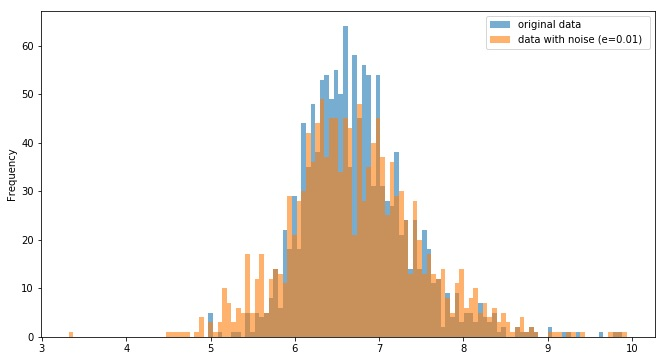
\includegraphics[scale=0.59]{images/hist001.jpg}
  \caption{Ιστόγραμμα συχνοτήτων των βαθμών}
  %\label{fig:boat1}
  \end{center}
\end{figure}

Βλέποντας τα δυο διαγράμματα συμπεραίνουμε ότι για $\epsilon=0.01$, ενώ η μέση τιμή είναι σχεδόν ανεπηρέαστη, θα υπάρχει σημαντική απόκλιση στα αποτελέσματα. Επιπλέον η διασπορά της κατανομής $Laplace$ οδηγεί στην εμφάνιση τιμών κάτω απο τη βάση του 5, πράγμα αδύνατον. 





\clearpage
\subsection{Πλήθος Τρίτεκνων}

Για τη συνέχεια των δοκιμών μας θεωρούμε το γνώρισμα "ΤΡΙΤΕΚΝΟΣ" ως ευαίσθητο, συνεπώς επερωτήσεις για συγκεκριμένες εγγραφές ως προς την τιμή του χαρακτηριστικού αυτού αποκλείονται. Μπορούμε, ωστόσο, να επερωτήσουμε συλλογικά τη βάση και να εξάγουμε συμπεράσματα. Τι γίνεται όμως στην περίπτωση που ένας επιτιθέμενος κατέχει πολύ μεγάλη γνώση για τα άτομα στην βάση?

H επερώτηση για το πλήθος των εγγραφών με θετική τιμή στο \textlatin{TRITEKNOS} επιστρέφει 32. Αυτό σημαίνει ότι η πιθανότητα ένα άτομο στη βάση να είναι θετικός στο γνώρισμα αυτό, είναι περίπου 2,3\%. Στη συνέχεια εφαρμόζουμε την επερώτηση «ποιό είναι το πλήθος των τρίτεκνων που έχουν βαθμό ίσο με 5». Η απάντηση είναι 1, ενώ το πλήθος των ατόμων με βαθμό 5 είναι τέσσερα. Η πιθανότητα επιλογής τρίτεκνου, δηλαδή, σε αυτό το υποσύνολο της βάσης είναι 25\%, δεκαπλάσια και πλέον από αυτήν επί του αρχικού συνόλου.

Υποθέτουμε τώρα ότι ο επιτιθέμενος γνωρίζει καλά τα περισσότερα άτομα στη βάση. Συγκεκριμένα ξέρει ότι ο Δημήτρης, η Φαίη και ο Ανδρέας έχουν βαθμό ίσο με 5 ακριβώς, ενώ είναι σίγουρος ότι κανείς τους δεν είναι τρίτεκνος. Σύμφωνα λοιπόν με τα παραπάνω δεδομένα, το τέταρτο άτομο του υποσυνόλου θα έχει θετική τιμή στο γνώρισμα. Προκύπτει λοιπόν αποκάλυψη του ευαίσθητου γνωρίσματος μιας εγγραφής.


\begin{figure} [h!]
\begin{center}
  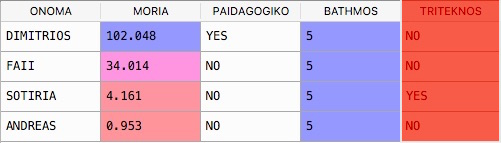
\includegraphics[scale=0.6]{images/tri1.jpg}
  \caption{Αποκάλυψη τιμής ευαίσθητου γνωρίσματος}
  %\label{fig:boat1}
  \end{center}
\end{figure}


Εφαρμόζοντας, ωστόσο, ελάχιστο θόρυβο με την μέθοδο της Διαφορικής Ιδιωτικότητας, βλέπουμε ότι η πιθανότητα αποκάλυψη της τιμής του γνωρίσματος "\textlatin{TRITEKNOS}" για μια εγγραφή είναι μηδενική.

Αν εισάγουμε θόρυβο στο γνώρισμα \textlatin{BATHMOS} όπως στην προηγούμενη παράγραφο, τότε θα είναι αδύνατο να εντοπιστούν τα 4 αυτά άτομα με βαθμό ίσο με 5. Βλέπουμε λοιπόν πως η διαφορική ιδιωτικότητα προστατεύει τα δεδομένα απο επιτιθέμενους με γνώση. 

Οι παραπάνω εφαρμογές δείχνουν ότι η εισαγωγή θορύβου στα δεδομένα και γενικά η τυχαιοποίηση είναι, θα τολμούσαμε να πούμε, η ασφαλέστερη επιλογή για την διατήρηση της ιδιωτικότητάς τους. Το μεγαλύτερο μειονέκτημα των μεθόδων αυτών είναι η επιλογή του ιδανικού μέτρου θορύβου ώστε να μην προκύψει διαστρέβλωση της πληροφορίας, ενώ ταυτόχρονα να είναι εγγυημένη η προστασία των δεδομένων. Συγκεκριμένα, στα παραπάνω παραδείγματα παρατηρήσαμε ότι η επιλογή της παραμέτρου $\epsilon$ είναι μια αρκετά επίπονη διαδικασία. Σχετικά με το θέμα αυτό έχουν γραφτεί πολλά άρθρα και έχουν προταθεί δεκάδες μέθοδοι οι οποίες αναζητούν τη «χρυσή τομή», χωρίς να προκύπτει πάντα το αναμενόμενο αποτέλεσμα από την εφαρμογή τους \textlatin{\cite{murtagh2016complexity}}. 